\documentclass[11pt]{article}
\usepackage[utf8]{inputenc}
\usepackage{lingmacros}
\usepackage{tree-dvips}
\usepackage{enumitem}
\usepackage{graphicx}
\usepackage[bottom]{footmisc}
\graphicspath{ {./images/} }

\title{Monitoring des données BRAMS et détection automatique des échos de météore}
\author{Miguel Antoons}

\begin{document}

\begin{titlepage}
    \begin{center}
        
\includegraphics[]{logo_ephec.png}\\
        \Large
        \textbf{Technologie de l'Informatique}\\
        \large
        Avenue du Ciseau 15\\
        1348 Ottignies
    \end{center}

    \vspace*{\stretch{1.0}}

    \begin{center}
        \line(1,0){350}\\
        \LARGE\textbf{Monitoring des données BRAMS et détection automatique des échos de météore}\\
        \line(1,0){350}\\
        \vspace{0.5cm}
        \LARGE\textit{Miguel Antoons}\\
        \vspace{0.5cm}
        \Large\textbf{Rapporteur}\\
        \Large\textit{Monsieur Arnaud Dewulf}
    \end{center}

    \vspace{0.14cm}

    \begin{center}
        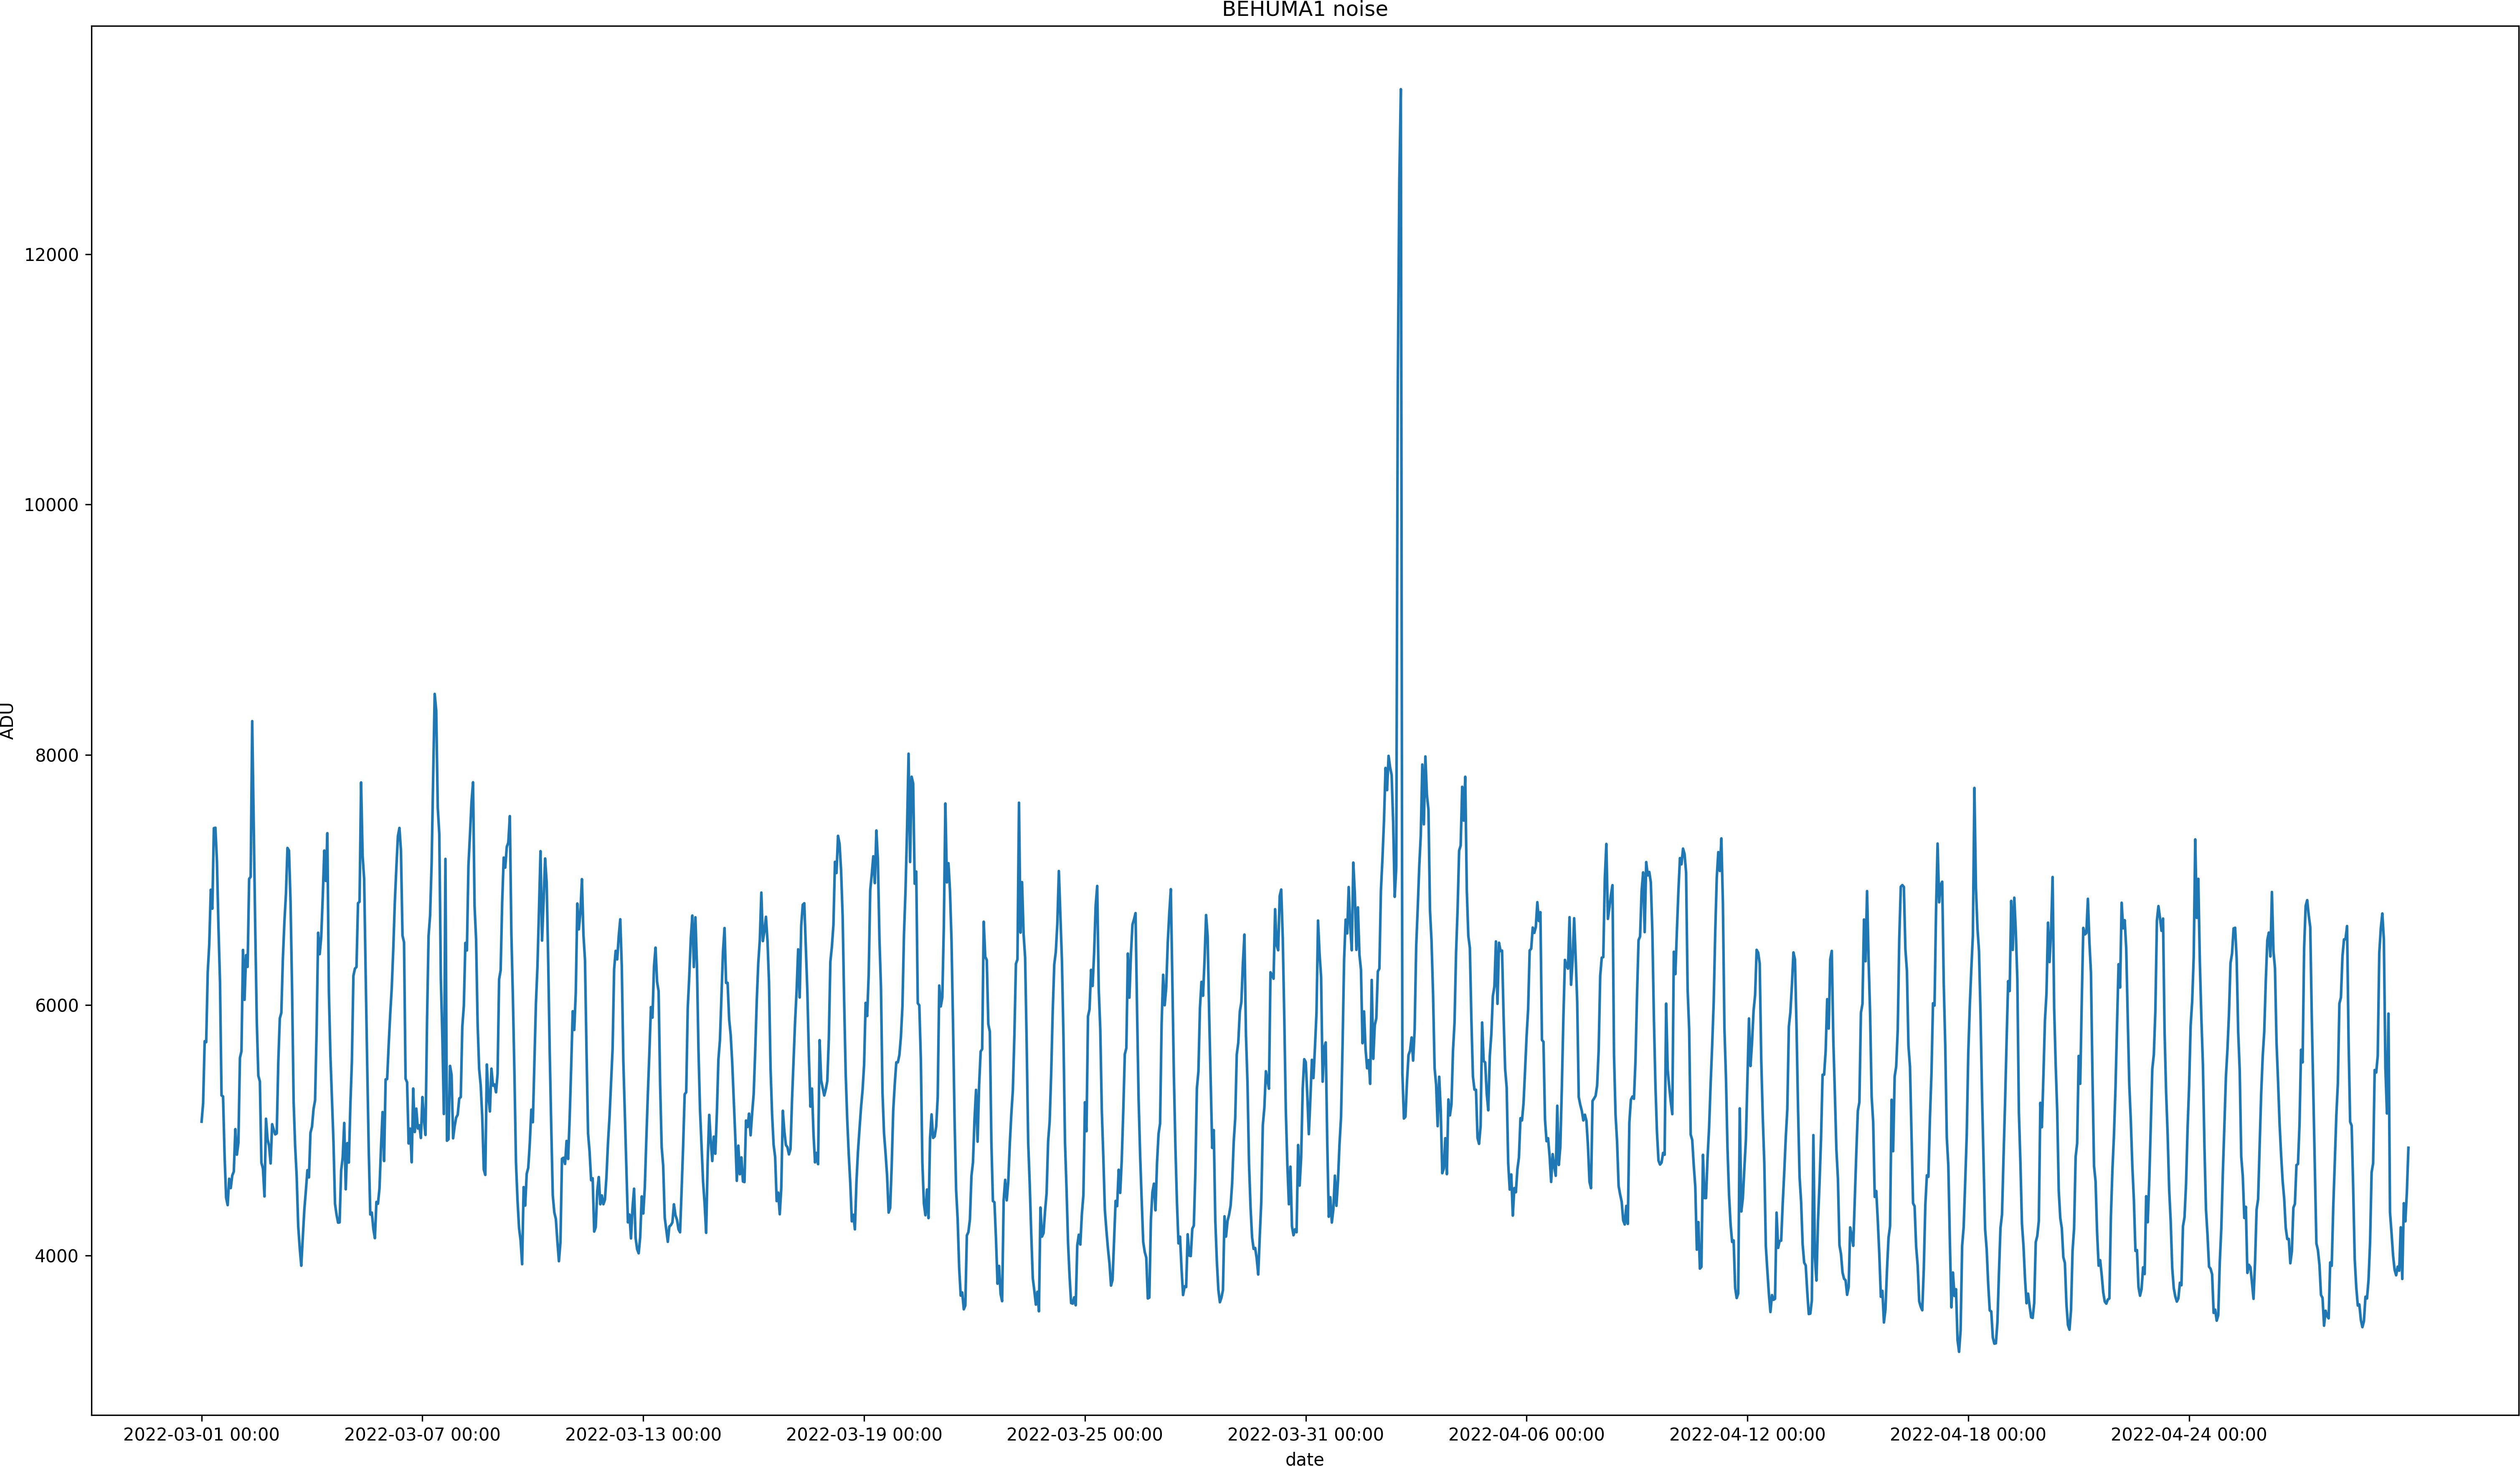
\includegraphics[scale=0.225]{page_garde.png}\\
        \vspace{0.14cm}
        \textit{2021-2022}
    \end{center}



    \vspace*{\stretch{2.0}}
\end{titlepage}

\tableofcontents

\newpage

\section{Remerciements}

Je tiens tout d'abord à remercier toutes les personnes qui m'ont aidé à réaliser ce projet de fin d'études.\\
\\
En commençant par mon professeur rapporteur, à qui j'ai pu poser mes questions en cas de besoin et qui s'est assuré que tout se passe bien tout au long du projet.\\
\\
Ensuite, je voudrai remercier Mr Hervé Lamy pour avoir proposé ce sujet de fin d'études, mais également pour m'avoir expliqué, de façon claire et précise, toutes les notions qui nécessitaient des explications.\\
\\
Je tiens également à remercier Mrs Antoine Calegaro et Michel Anciaux, qui m'ont guidé quand c'était nécessaire et qui m'ont conseillé durant le projet de fin d'études.\\
\\
Enfin, je voudrais exprimer ma reconnaissance envers toutes les personnes qui m'ont conseillé sur, et ont relu ce rapport de projet de fin d'études.

\end{document}